%!TEX root = ../PatilM-[RnD-MT]Report.tex

\chapter{State of the Art}
\paragraph{}Over the years, research into qualitative spatial representations has led to the development of various models which can be used to represent the visually observable space.From a more scientific perspective these models are known as `Qualitative calculi', the current state of the art calculi rely on a single spatial primitive such as distance, direction, topology etc., to describe a set of relationships amongst the observable objects. In general each calculi comes with its own set of benefits and drawbacks as each one of them has been tailored to exploit different aspects of space\cite{chen2015survey}, \cite{cohn2008qualitative}. 

\paragraph{}For the case of robot navigation, current state of the art approaches utilize qualitative calculi that can provide both spatial and temporal information such as the QTC \cite{van2005qualitative} or QRPC \cite{glez2013qrpc}. There exist comprehensive surveys that provide detailed information about each of the existing qualitative calculi\cite{cohn1997qualitative}, \cite{chen2015survey}, \cite{cohn2001qualitative}, \cite{cohn2008qualitative} hence this state of the art aims to provide only a concise overview of the qualitative calculi that are advantageous to our application. We shall look into the relationships afforded by each of these calculi and their classification based on the domain of their utility.

 
\section{Forms of qualitative spatial representations}
		%    \item \textcolor{blue}{What have other people done?}
		%    \item The work presented in Alan Blackwell's master thesis \cite{blackwell1988spatial} provides a qualitative method for  representation of two dimensional shape and position and has been used to solve a few simple spatial reasoning tasks, with applications in the field of robotics. While the focus is mainly on the development of a qualitative representation it doesn't particularly focus on the use of this method for robot navigation. The outlined approaches for the use case in robot navigation raises more questions instead of providing a solid practical approach to the problem. 
		
		
		%    \item \cite{chao2014survey}
		%	\item \cite{dondrup2015computational}
		
		\subsection{Topological Representations} : This is the most fundamental spatial representation\cite{cohn1997qualitative}, \cite{chen2015survey} wherein the observed space is divided into distinctive regions based either on distinctive points in space or on separable objects found in the space. Topological representations draw heavily from the field of ``Mereology''(the theory of parthood) to describe relations between the distinctive regions \cite{cohn2001qualitative}, \cite{cohn2008qualitative}. Qualitative calculi such as RCC, Interval Algebra, n-intersections etc. belong to this category. Such representations deal with the `\textit{invariant properties that are under continuous deformations of objects, including translating, rotating and scaling}', and often include only spatial information while completely disregarding temporal data. 
		
		\begin{figure}[h]
			\centering
			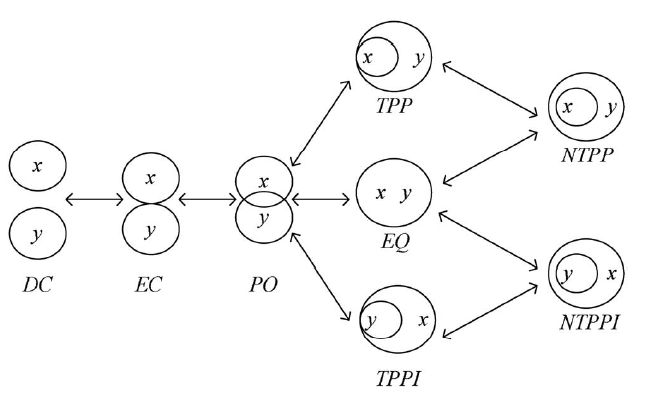
\includegraphics[width=0.7\linewidth]{images/rcc8_rel}
			\caption{The eight jointly exhaustive and pairwise disjoint relations of region connection calculus (RCC8). The arrows show which relation is the next relation a configuration would transit to, assuming the continuous movements or deformations \cite{cohn1997qualitative}, \cite{chen2015survey}, \cite{cohn2001qualitative}, \cite{cohn2008qualitative}.}
			\label{fig:rcc8rel}
		\end{figure}
		
		
		\subsection{Directional Representations}: The relative direction between two different objects can be represented using directional relations/representations \cite{cohn1997qualitative}, \cite{chen2015survey}, \cite{cohn2001qualitative}, \cite{cohn2008qualitative}. These representations rely on three primary elements, a reference object, a reference frame and a target object to define a valid relation between two different objects. Directional representations are widely classified into two categories, point based and projection based with the discerning factor being the dimension of the objects involved and distinction of space using either cone shaped spatial sectors or by using vertical and horizontal lines to create smaller rectangular sectors. Furthermore, the directional calculus isn't restricted to using only cardinal directions, it also allows the use of nominal directional information such as left, right etc. to describe the directional relations. Qualitative calculi such as CDC, OPRA, CyCord etc. utilize the directional representation. Being based of topological representations, directional representations also include only spatial information while disregarding temporal data.
		
		\begin{figure}[h!]%
			\centering
			\subfloat[Cone-shaped direction relations \cite{isli2000new}]{{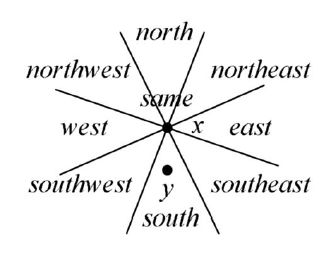
\includegraphics[width=6cm]{images/direction_cone} }}%
			\qquad
			\subfloat[Projection-based direction relations \cite{isli2001combining}]{{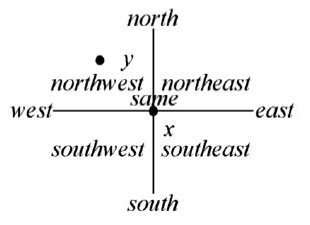
\includegraphics[width=6cm]{images/direction_projection} }}%
			\caption{The point based and projection based direction representations \cite{chen2015survey}}%
			\label{fig:example}%
		\end{figure}
	
		\subsection{Distance Representations}: The qualitative representation of spatial distance can be classified into two groups namely absolute and relative \cite{isli2000new}, \cite{chen2015survey}, \cite{cohn2001qualitative}, \cite{isli2001combining}. This classification is made solely on the basis of  the presence/absence of an extraneous referential object in the relation between two objects. This distinction can be clearly illustrated by the following example,`the distance between A and B is 8 meters' or `A is near B', this is a absolute approach as the distance is measured directly between two objects.Whereas saying that `A is closer to B than that to C' classifies as a relative approaches as this involves the comparison to a third object. Furthermore, it has been shown that absolute approaches	can be qualitative or quantitative, but relative approaches are commonly qualitative \cite{cohn2001qualitative}.Qualitative calculi such as the ARGD (or Delta) and TPCC use the distance representations to describe the observable space. Distance based relations have found to be insufficient by themselves when it comes to the task of robot manipulation/navigation and hence are often used in combination with distance representations to yield a fairly suitable and complete representation of the environment \cite{chen2015survey}. Like with the direction representations this calculi also lacks temporal data in the encoded relations and is hence unsuitable for applications involving moving objects.
		
		\begin{figure}[h]
			\centering
			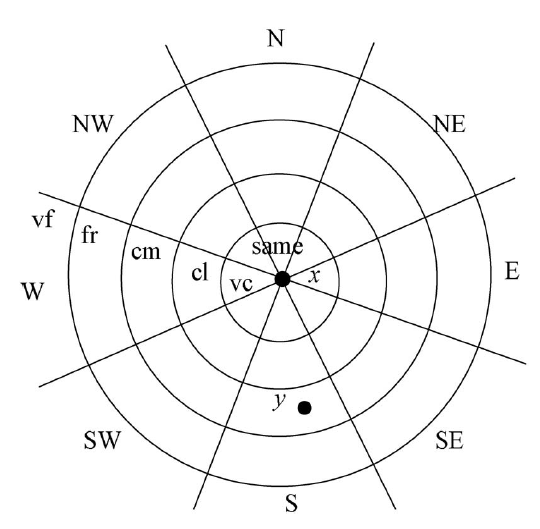
\includegraphics[scale=0.8]{images/argd_delta}
			\caption{An representation of the combination of cone-shaped direction and absolute distance: very
				close(vc), close(cl), commensurate(cm), far(fr) and very far(vf), \cite{clementini1997qualitative}.}
			\label{fig:argddelta}
		\end{figure}
		
		
		\subsection{Moving object Representations}  Topological representations, directional representations
		 and distance representations describe relations between stationary objects. This limitation encouraged the development of a moving object representation which can qualitatively represent moving objects and their trajectories \cite{cohn1997qualitative}, \cite{chen2015survey}, \cite{cohn2001qualitative}, \cite{cohn2008qualitative} . These representations effectively deal with both spatial and temporal data to describe valid relations among mobile objects. While these relations include some directional information they mainly describe the relative motion between two objects and not relative direction. The relative motion between two objects is described using oriented line segments which are approximations of the trajectory of the objects in motion. QTC, QRPC are the two prominent calculi that utilize moving object representations. Moving object representations and the calculi using these representations have been proven to have solved the problem of representing moving objects but since these relations lack any distance information, they are still prone to failure and often need a complimentary distance calculi to ensure that a mobile object(robot) can successfully move around in the given environment without collisions.
		
		\begin{figure}[h]
			\centering
			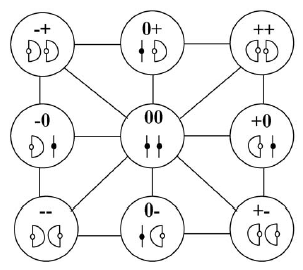
\includegraphics[scale=1]{images/qtcb}
			\caption{Basic relations of basic Qualitative Trajectory Calculus (QTCB) in a conceptual neighborhood diagram. The solid dots represent the stationary objects and the open dots represent the moving objects \cite{bibid}, \cite{de_weghe}.}
			\label{fig:qtcb}
		\end{figure}		
		
		\newpage
		
		\begin{table}[h!]
			\begin{adjustwidth}{-2cm}{}
				\resizebox{\textwidth}{!}{%
					\begin{tabular}{|p{3cm}|p{4cm}|p{3cm}|p{8cm}|}
						\hline
						\textbf{Domain} & \textbf{Model Name} & \textbf{Type of objects} & \textbf{Description} \\ \hline
						\multirow{2}{*}{Temporal} & Interval Algebra \cite{allen1990maintaining} & Time Intervals & It does not consider time instants. \\ \cline{2-4} 
						& Extended Interval Algebra  \cite{freksa1992temporal} & Time intervals and extreme points of the intervals & It extends IA(Interval Algebra) model by considering new relationships including the extremes of the interval and it introduces the notion of conceptual neighborhood. \\ \hline
						\multirow{8}{*}{Spatial} & Region Connection Calculus  \cite{randell1992spatial} & Sets & It uses the geometric properties associated to the connection between two sets to establish relationships that are no longer linear but planar, and which are invariant to translation, rotation and scaling. \\ \cline{2-4} 
						& Cardinal Reference System(CRS)  \cite{frank1992qualitative} & Generic objects & It describes the position of any object by using a cardinal orientation as reference system and by adding also a neutral region \\ \cline{2-4} 
						& FFC (Flip Flop Calculus) \cite{ligozat1998reasoning} & Points & It is based on the possible positions of a point C with respect to a segment AB defined by other two points, A and B. \\ \cline{2-4} 
						& SCC (Single Cross Calculus) \cite{freksa1992temporal} & Points & Describes the possible positions of a point C with respect to a segment AB and the orthogonal line to segment AB on B. \\ \cline{2-4} 
						& DCC (Double Cross Calculus)  \cite{freksa1992utilization} & Points & Describes the possible positions of a point C with respect to a segment AB and two orthogonal lines to segment AB on A and B. \\ \cline{2-4} 
						& Oriented point based Reasoning  \cite{moratz2006representing}& Oriented Points & It is based on the relative orientation between pairs of oriented points in terms of two qualitative spatial dichotomies: the front–back and left–right. \\ \cline{2-4} 
						& DRA (Dipole Relation Algebra)  \cite{dylla2004empirical}, \cite{dylla2004exploiting} & Dipoles (or oriented segments) & It is based on the relative position of oriented segments. \\ \cline{2-4} 
						& OPRA (Oriented Point Relation Algebra)  \cite{dylla2006generalizing} & Oriented points & As DRA model, it is also based on the relative position two oriented points, but it supports different levels of granularity. \\ \hline
						\multirow{2}{*}{Spatio-temporal} & QTC (Qualitative Trajectory Calculus)  \cite{van2005representing} & Points & It describes the possible relations among two moving points in terms of the front–back and left–right dichotomies. \\ \cline{2-4} 
						& QRPC (Qualitative Rectilinear Projection Calculus)  \cite{glez2013qrpc} & Oriented points & It establishes the possible relations of an object with respect to the trajectory of another object depending on the cross-point of the trajectories and the relative position among them \\ \hline
				\end{tabular}}
			\caption{Table(from \cite{glez2013qrpc}) describing the key features of the more representative models(calculi) of qualitative representations of spatial or temporal domains in the existing literature.}
			\end{adjustwidth}
		\end{table}
	
			\newpage
	
		\subsection{Conclusion}From the above breakdown of the representations and the calculi, it is easy to summarize that distance representations and moving object representations are the most promising representations for our application in mobile robot navigation \cite{chen2015survey}, \cite{cohn1997qualitative}. Consequently the calculi associated with these representations will be the ones that are further scrutinized in the following section. The reasoning behind this conclusion is fairly simple moving object representations are basically spatio-temporal \cite{cohn2001qualitative}, \cite{cohn2008qualitative}, \cite{Yan2012QualitativeRA} representations which take into account both the spatial and temporal data to create abstractions of the objects trajectory, this is crucial when dealing with mobile objects as this gives a more concrete representation of the objects in motion \cite{glez2013qrpc}. In the case of distance representations although these representations deal only with spatial information, they provide explicit information on how close or far the objects under consideration are. Thus effectively capturing the possibility of a collision between the objects, this sort of information cannot be found in the direction and topological representations hence rendering them unfavorable for our application in mobile robot navigation  .
	
	\section{Analyzing qualitative calculi for navigation}
	\paragraph{} This section aims to provide a thorough understanding at a selective group of qualitative calculi based on the conclusions drawn from the previous section. Namely we shall look at the qualitative calculi such as the QTC, QRPC and ARGD which use moving object representations and distance representations and function in the spatio-temporal and spatial domains respectively.
%	write only theory here
	\subsection{Qualitative Trajectory calculus}
	\paragraph{}The QTC calculus was developed to solve the problem of inadequate representation of mobile objects in the spatio-temporal domain, which until then were represented only in the spatial domain using either the RCC or the n-intersections calculi \cite{van2006qualitative}, \cite{van2005qualitative}. The major drawbacks of those calculi was their failure to deal with temporal data. Hence mobile objects were often abstracted as stationary regions using either 'disconnected from' relation (DC) in RCC or 'disjoint' relation in the 9-intersection model, with the exception of a few limiting cases where the two objects meet, such as a collision between two mobile robots \cite{van2004representing}. Thus, the limiting factor of these formalisms was that all the DC relations were non-differentiable, due to the ignorance of information regarding relative motion between the two objects .
	\paragraph{}The QTC calculus constitutes of two major variants the $QTC_B$ and the $QTC_C$, with the major difference between the two being the inclusion of the directional information in the relationships (between two objects) of the $QTC_C$ calculus. Both versions of the QTC are adept at dealing with qualitative movement of objects in one, two and three dimensions. The $QTC_B$ calculus, takes Euclidean distance between two objects as the only constraining dimension.The abstraction of movement is depicted using three qualitative values:
	\begin{itemize}
		\item 0: the object is stable with respect to the other object.
		\item -: the object is moving towards the other object.
		\item +: the object is moving away from the other object.
	\end{itemize}
	The assigning of these qualitative values to an object's movement depends upon the relative position (constrained by distance) and relative speed of the two objects with respect to each other. This can be illustrated by the following example, consider two objects `j' and `k', the possible values for `j' :
	
	\begin{itemize}
		\item based on relative position at a time `t' are:
		\begin{enumerate}
			\item 0 (stable): if there is no change in the relative position with respect to `k' (no change in relative distance ).
			
			\item - (moving towards): if there is a change in the relative position with respect to `k', such that the relative distance between the objects decreases.
			
			\item + (moving away): if there is a change in the relative position with respect to `k', such that the relative distance between the objects increases.
		\end{enumerate}
		\item based on relative speed at a time `t' are:
		\begin{enumerate}
			\item 0 (stable): if speed of `j' is equal to the speed of `k'.
			
			\item - (moving towards): if speed of `j' is lesser than the speed of `k'.
			
			\item + (moving away): if speed of `j' is greater than the speed of `k'.
		\end{enumerate}
	\end{itemize}

	\paragraph{}Hence a valid $QTC_B$ relation between qualitative trajectories of two objects is represented as such `{-,+,-}'(for object 1 with respect to object 2) and `{+,-,+}' (for object two with respect to object 1)%since these relations are always mirrored, sets of such relationships can be easily defined for either object depending upon the object in focus%
	. In each individual relationship the value in the first position is the relative position of the object in consideration, the second value is the relative position of the other object and the third value is the relative speed of the current object with respect to the other object. The benefit of having a relation that includes both relative position and speed comes to light when dealing with the movement of objects in higher dimensions (2D, 3D). For instance in 2D, the value `0'(stable) may be interpreted as either the distance being stable or the speed being stable, this confusion during interpretation is avoided by using unique values for both the relative distance and speed and hence the size of the resulting relations is a set of three. Interpretation of these relations is pretty straight-forward when dealing with movements one dimension. The $QTC_B$ being developed to deal with mobile objects when they are exclusively in DC (dis-connected) regions \cite{van2006qualitative} makes it susceptible to inaccuracies when building relations regarding collision conditions.
	
	\paragraph{}The $QTC_C$ variation of the QTC calculus is often seen as an extension of the $QTC_B$ calculus, since it uses the same qualitative values to represent the qualitative trajectories of the objects. The only difference between the two versions comes from the integration of directional information which denotes the direction of movement of the current object in relation to a line segment between the two objects. This version of the QTC calculus was inspired in part by the `Double cross calculus' \cite{zimmermann1996qualitative}, hence the name. The $QTC_C$ calculus is an improvement on the double cross calculus, as it can define qualitative trajectories and direction for single as well as multiple objects at once, whereas the double cross calculus can only deal with single objects at any given instance of time.
	
	\newpage
	
	\begin{figure}[h!]
		\centering
		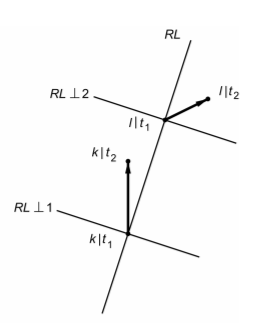
\includegraphics[scale=1]{images/QTCC}
		\caption{A graphical representation of the $QTC_C$ calculus for a relation between two moving objects`k' and `l', where $t_1$ and $t_2$ are the two distinctive time instances and RL refers to the reference line and the double crosses($RL\perp1$, $RL\perp2$) for the two objects \cite{van2005qualitative} .}
		\label{fig:qtcc}
	\end{figure}

	\paragraph{}The relations of the $QTC_C$ calculus, while following the same basic principles of the $QTC_B$, have been tweaked slightly to allow inferencing of the objects position in terms of the relative direction to the reference line. The assignment of the qualitative values to the object's movements can be illustrated using two objects `k' and `l', the possible values for `l' at any given time interval are based on the following reasoning:
	
	\begin{itemize}
		\item based on movement relative to the respective perpendicular reference line:
		
		\begin{enumerate}
			\item 0 (stable): if there is no change in the relative distance with respect to `k' or with respect to the reference line. 
			
			\item - (moving towards): if there is an increase in the relative distance between the objects.
			
			\item + (moving away): if there is an increase in the relative distance between the objects.
		\end{enumerate}
	
		\item  based on movement relative to the directed perpendicular reference line(from `l' to `k'):
		
		\begin{enumerate}
			\item 0 (moving along the directed reference line): if the object moves
			along the line segment or if it was moving along the left/right and continues to do so in the given time interval.
			
			\item - (moving to left side of the directed reference line): if the object moves from the right side of the line segment to the left side in the given time interval.
			
			\item + (moving to right side of the directed reference line): if the object moves from the left side of the line segment to the right side in the given time interval.
		\end{enumerate}
	
	\end{itemize}

	\paragraph{}Hence a valid $QTC_C$ relation between qualitative trajectories of two objects is represented as such `{-,+,-,0}'(for object 1 with respect to object 2) and `{+,-,0,-}'(for object 2 with respect to object 1). Wherein the value in the first position is the relative movement(towards-away) of the object in consideration, the second value is the relative movement(towards-away) of the other object, the third value is the relative direction(left-right) of movement of the first object and the fourth is the relative direction(left-right) of movement of the second object.
	
	\paragraph{Conclusion}To conclude, the $QTC_B$ calculi is a basic and restrictive representation that encodes only the motion of the object and not its direction of movement. Yet, this restriction allows for a more assured set of relations that do not encode any ambiguity corresponding to the relative motion of the objects in question \cite{van2004representing}. The $QTC_C$ on the other hand does not provide distinctive relations to distinguish between the trajectories of a mobile object moving along the directed reference line and continuing to do so and a mobile object moving on either side of the directed reference line and continuing to do so \cite{van2005qualitative}. Therefore leading to a rather ambiguous interpretation of the direction of the object's relative motion, factor into this the fact that we will implement it on a robot in a live environment and it becomes clear that there will be numerous cases of collision that could endanger the safety of the robot as well as the other agents that lie in its vicinity.  Hence justifying the selection of $QTC_B$ for our implementation, not only is it safer and simpler but it also allows easier integration with other complimentary calculi such as ARGD, RCC which may be used to deal with possible collision cases.

	\subsection{Qualitative Rectilinear Projection calculus}
	\paragraph{}The qualitative rectilinear projection calculus (QRPC) \cite{glez2013qrpc}, \cite{alvarez2006guide},  \cite{delafontaine2011implementing} presents an innovative approach to qualitatively representing motion patterns based on planar trajectories. In comparison to the QTC calculus, this representation has a richer description of the motion exhibited by mobile objects. The basis of this claim lies in the oriented rectilinear projection used to represent the trajectories, which allows this calculus to represent rotational motions of an mobile object, something that was not possible in the existing calculi such as the QTC. The QRPC is specifically tailored towards obstacle avoidance and geometric relationships between two objects are generated using the front-back and the left-right dichotomies. The relationships encompassed in the QRPC abstract the objects as points and use their rectilinear projections to make qualitative distinctions such as front-back and left-right, these atomic relations and their base notations are illustrated below:
	
	\begin{enumerate}
		\item \textbf{Notations:}
		
		\begin{itemize}
			\item $P_iP_j$: is the relative disposition between the oriented rectilinear	projection of the object $O_i$ and the oriented rectilinear projection of $O_j$.
			\item $O_iO_j^{LR}$: The relative position of $O_i$ with respect to the left-right dichotomy of $O_j$.
			\item $({CO_i}^{FB})({CO_j}^{FB})$: The relative position of the point of intersection(`C') of the oriented rectilinear projections with respect to the front–back dichotomy of both objects.
			\item $O_iO_j^{FB}$:  The relative position of $O_i$ with respect to the front-back dichotomy of $O_j$ when the trajectories are superimposed.
			
			Note: `i' and `j' denote the two different objects.
		\end{itemize}
		
		\item \textbf{Qualitative relations (atomic) in each of the notations :}
		\begin{itemize}
			\item The relative disposition between two oriented rectilinear projections($P_iP_j$):
			
			\begin{itemize}
				\item  $\uparrow \uparrow$  : Parellel in same direction
				\item $\uparrow \downarrow$  : Parellel in opposite direction
				\item $\uparrow$  : Coincident in same direction
				\item $\updownarrow$  : Coincident in opposite direction 
				\item $X$  : Crossed/Intersecting rectilinear projections 
			\end{itemize}
		
			\item The relative position of $O_i$ with respect to the left-right
			dichotomy of $O_j$, ($O_iO_j^{LR}$):
			\begin{itemize}
				\item `-' : if $O_i$ is on the left of $P_j$.
				\item `0' : if $O_i$ is over $P_j$.
				\item `+' : if $O_i$ is on the right of $P_j$.
				
				\begin{figure}[h]
					\centering
					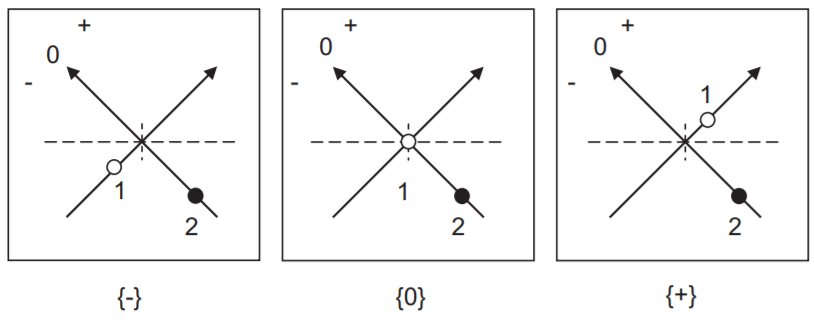
\includegraphics[width=0.7\linewidth]{images/QRPC_FB}
					\caption{Relative position of $O_i$(object 1) w.r.t the left-right dichotomy of $O_j$(object 2) for crossed projections \cite{glez2013qrpc}.}
					\label{fig:qrpcfb}
				\end{figure}
				
			\end{itemize}
			
			\item The relative position of `C' with respect to the front-back
			dichotomy of two objects $(CO_i^{FB})(CO_j^{FB})$:
			\begin{itemize}
				\item $(+,+)$ : if `C' is in front of $O_i$ and $O_j$.
				\item $(0,+)$ : if `C' is at same position as $O_i$ and in front of  $O_j$.
				\item $(+,-)$ : if `C' is in front of $O_i$ and behind $O_j$.
				\item $(0,-)$ : if `C' is at same position as $O_i$ and behind $O_j$.
				\item $(-,+)$ : if `C' is behind $O_i$ and in front of $O_j$.
				\item $(-,0)$ : if `C' is behind $O_i$ and in same position as $O_j$.
				\item $(-,-)$ : if `C' is behind $O_i$ and $O_j$.
				\item $(+,0)$ : if `C' is in front of $O_i$ and at the same position as $O_j$.
				\paragraph{}In cases where the two projections do not intersect with each other($\uparrow \uparrow$ or $\uparrow \downarrow$), this qualitative abstraction presents as conundrum as the point of intersection `C' may lie at either positive or negative infinity, hence in such cases the relation is abstracted to either $(+,+)$ or $(-,-)$.
				
				\begin{figure}[h]
					\centering
					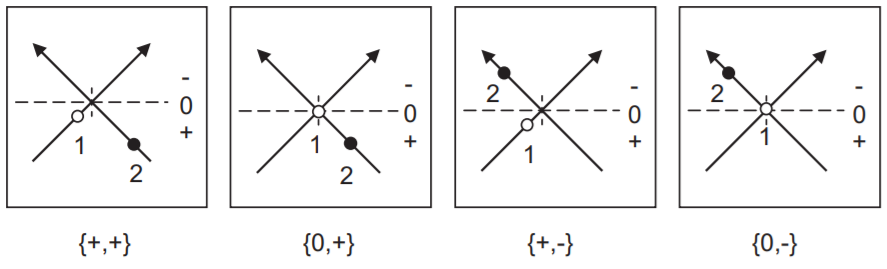
\includegraphics[width=0.7\linewidth]{images/QRPC_PJ}
					\caption{Some of the spatial configurations of the intersection point with respect to the front-back dichotomy of two objects for crossed projections $(CO_i^{FB})(CO_j^{FB})$, \cite{glez2013qrpc}.}
					\label{fig:qrpcpj}
				\end{figure}
				
			\end{itemize}
		\item The relative position of $O_i$ with respect to the front-back dichotomy of $O_j$ when the trajectories are superimposed($O_iO_j^{FB}$):
		\begin{itemize}
			\item `+' : if $O_i$ is in front of $O_j$ after $P_i$ is superimposed on $P_j$.
			\item `0' : if $O_i$ is at the same position as $O_j$ after $P_i$ is superimposed on $P_j$.
			\item `-' : if $O_i$ is behind $O_j$ after $P_i$ is superimposed on $P_j$.	
			
			
			Note: The after the rectilinear projection of $O_i$ is rotated(such that the objects are always facing in opposing directions) along `C' if it exists, before being superimposed on the rectilinear projection of $O_j$.		
		
			\begin{figure}[h!]%
				\centering
				\subfloat[The ($O_iO_j^{FB}$) feature for crossed projections. \cite{glez2013qrpc}]{{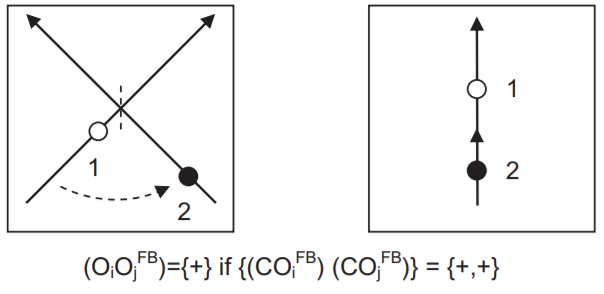
\includegraphics[width=6cm]{images/QRPC_ob1} }}%
				\qquad
				\subfloat[The ($O_iO_j^{FB}$) feature for parellel projections. \cite{glez2013qrpc}]{{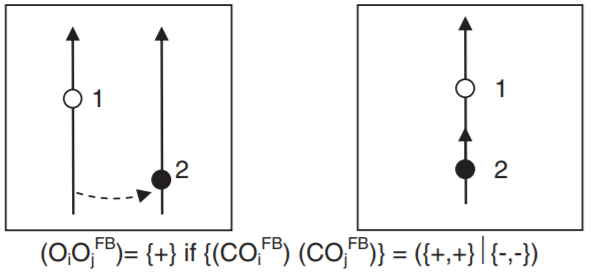
\includegraphics[width=6cm]{images/QRPCob2} }}%
				\caption{The point based and projection based direction representations \cite{glez2013qrpc}}%
				\label{fig:QRPC superimposed}%
			\end{figure}
			
		\end{itemize}
	
		\end{itemize}
	\end{enumerate}
	\paragraph{Conslusion}Hence a complete valid QRPC relation comprising of the above mentioned atomic relations can be written as [($P_iP_j$)($O_iO_j^{LR}$)($({CO_i}^{FB})({CO_j}^{FB})$)($O_iO_j^{FB}$)], with the various values replacing their respective placeholders. Thus proving to be a richer representation of the movements of the mobile objects as it can effectively distinguish  between front-back, left-right as well as same or opposing direction of heading. While this calculus does present a compact view of the movements of the objects, like its predecessors it still requires a sequence of qualitative(QRPC) states(individual sets of relations) to effectively represent the movement of an object. Besides, a completely theoretical formulation of the calculi specifically for GIS, limits its utility in robotics as there is no clear indication of the changes that need to be effected to ensure a reliable approach for mobile robot navigation. These drawbacks dissuade us from further pursuing this calculi for our purpose of achieving qualitative perception and control in mobile robots \cite{glez2013qrpc}. 
	
	\subsection{Qualitative Distance Calculus}
	\paragraph{} The qualitative description of distance is based on three primary elements, a primary object, a reference object and a reference frame \cite{clementini1997qualitative}, \cite{zimmermann1996qualitative}. When making a statement such as `A is near B' the qualitative inference is ambiguous without taking into consideration spatial entities such as metric distance between the objects, their respective sizes and shapes, their relative positions, the positions of other objects as well as the frame of reference with respect to the objects itself. Furthermore the distance between two objects varies with perspective, for instance looking at a moving object from two different perspectives leads to two different interpretations of the distance to the object, with respect to observing entity. The distance calculi aims to summarize all these varying spatial quantities into a single coherent qualitative description which can be used to reason about space in terms of qualitative distances.
	\paragraph{}The ARGD or Delta calculus are some of the common names used for the qualitative distance calculus. These calculi partition the physical space into circular regions of varying granularity. Since there is no restriction on the number of granular divisions that can be applied to a given physical space we may define this in a manner that is suitable for our application. Commonly the granularity varies from anywhere between 2-5, with the respective labels being very close, close, commensurate, far, and very far.
	
	\begin{figure}[h]
		\centering
		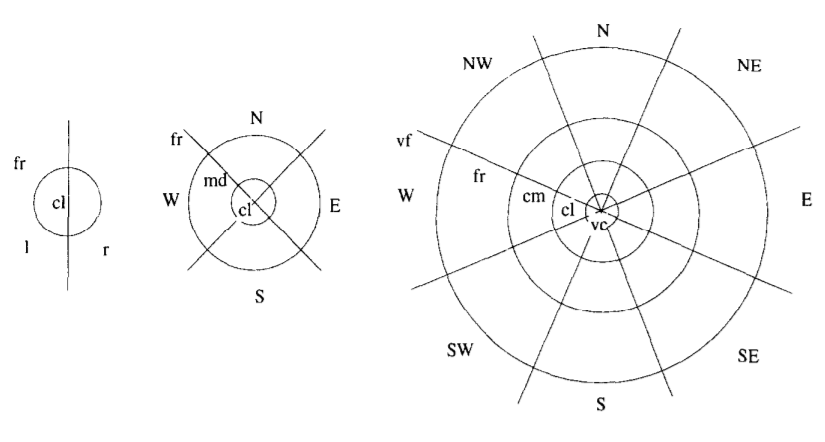
\includegraphics[width=0.7\linewidth]{images/distance_cal}
		\caption{ Various levels of distance and orientation distinctions. These figures show typical distance/orientation granularity configurations \cite{clementini1997qualitative}. }
		\label{fig:distancecal}
	\end{figure}
	
	\paragraph{} The various granular regions in the distance calculi are always centered around the object in consideration, these granularities are subject to an inherent `greater than' order amongst themselves such that the granular region closest to the object has the lowest distance value and the one that is farthest has the highest order. Consider `$q_n$' as the granularity of the distance representation, then the various instances are organized as such [$q_0 < q_1 < q_2 < . . . < q_n$], with $q_0$ being the smallest distance to the object and $q_n$ being the largest. By using this comparative approach for distance magnitudes the calculus effectively maps the granular symbols to one dimensional geometric intervals that represent the distance ranges.
	
	\paragraph{Conclusion}Since the applicability of the distance approach does not depend upon the number of distance relations \cite{clementini1997qualitative}, it allows the distance calculus to be highly adaptive to the users demands and hence provides a feasible alternative to collision free navigation in mobile objects. Also as mentioned previously the distance representation effectively divides the physical regions around the object into geometric intervals, hence making this approach suitable to define distance thresholds around the robot to avoid collisions with other objects as well as define a suitable safe region around the robot \cite{lowe1975geography}, which in-turn ensures safe movement in the physical space. These benefits of the qualitative distance calculi make it favorable to our application, hence warranting its utilization.

	\section{Implementations utilizing qualitative representations for navigation in robots}
	\paragraph{} The goal of this section is to introduce the reader to the existing approaches that use qualitative spatial representations in some capacity to achieve efficient and collision free navigation in mobile robots. The merits and de-merits of each implementation is recognized and a brief summary is constructed based upon the same.
	
	
	 This approach \cite{chen2006qualitative}, relies heavily on the detection of tangible features in two sets of images one of which is a reference image that is taken during a teach phase (when the robot is taken manually through the desired path and allowed to take reference images through out its path traversal) and a second image that is taken during a replay phase during which the robot is allowed to navigate the desired path by itself, capturing new images all along. The features in both these images are detected and tracked using the Kanade-Lucas-Tomasi \cite{birchfield2007klt} feature tracker. The tracked features in the current image (taken during the replay phase) are compared with the features observed in the reference image (taken during the teach phase) and the difference in their positions and distance is used to make qualitative decisions regarding the corrections that have to be made to the robot's path with respect to the desired path.
	The underlying spatial entity that is compared is the corresponding distance between the tracked features (in both the reference and the current image and the reference image) with respect to a common principal point of the images. Based on this conditions the decisions are made as follows:
	\begin{itemize}
		\item if the robot is moving from point A to B without deviating from the original path, then continue the current path until some deviation occurs.
		\item if the robot deviates laterally from the desired path and this is indicated in the signed distances between the features of the current and reference image, then:
		\begin{itemize}
			\item if the distance between the reference feature lying on the left/right of the image and the principle point is more than the distance between the current feature lying on the left/right of the image and the principle point then move left or right respectively.
			\item if the signed distance of the feature lying on the left/right of the image does not match with the sign of the feature lying on the left/right of the reference image then move right or left respectively.
		\end{itemize}
	\end{itemize} 
	\paragraph{Conclusion}The merits of such an feature based approach \cite{chen2006qualitative}, seem to be apparent, yet this approach does not utilize any of the traditionally accepted qualitative calculi. Furthermore its reliance on a teaching phase renders it invalid in cases where prior information about the environment is denied to the robot. The dependence on further factors such as lighting conditions, detection of features and inability to work efficiently in an outdoor environment(due to lack of contrast, the features are not detected) show that this is a highly constrained approach that can work only if a large amount of prerequisites are satisfied. The merit of this approach is still its ability to function exceptionally well when the teach phase is executed properly, with the robot able to follow trajectories upto a 100 meters easily. The authors also mention the apparent improvement in efficiency(in terms of 	reduced cost and power consumption as well as increased robustness) when using such qualitative approaches,  but fail to provide empirical proof for such statements.
	
	\paragraph{}The approach presented in \cite{chen2009qualitative}, also utilizes detection of tangible features to extract pixel coordinates of these features and then compare these coordinates with the corresponding pixel coordinates of the feature in the reference frame. The resulting differences are then used to make decisions regarding the control of the robots trajectory, as previously introduced this approach also makes use of the teach-replay method. This paper extends the approach presented in \cite{chen2006qualitative} by combining the pixel coordinates with odometry information to achieve a more robust navigation, also the use of the `funnel lane' methodology is a novel concept that helps in localizing the robot. The underlying spatial entity used in this approach is the relative positions of the features with respect to the principal point of the image, which yields signed (x,y)co-ordinate values. The distance between these reference points and the principal points is used to define a region called the `funnel lane', while the robot lies in this region it is allowed to move directly towards the goal position, but if there are any violations such that the robot moves out of this `funnel lane' then the controller updates the control commands to ensure the robot re-enters the `funnel lane'. Since the `funnel lane' is oriented such that its origin is always at the goal position hence ensuring that the robot zeros in on the goal position.
	\begin{figure}[h]
		\centering
		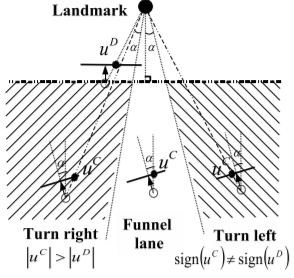
\includegraphics[scale=1]{images/funnel_lane}
		\caption{The funnel lane created by the two constraints(distance from the principal point and the relative signs of the distances), and when it has turned by an angle $\alpha$, here $\mu^C$  and  $\mu^D$ represent the horizontal pixel coordinates of the reference and the current frame \cite{chen2006qualitative}.}
		\label{fig:funnellane}
	\end{figure}
	
	\paragraph{Conclusion}Being an extension of the approach specified in \cite{chen2006qualitative}, this implementation \cite{chen2009qualitative}, suffers from very much the same over-reliance on the teach phase to correctly capture the reference features, while completely failing to utilize any of the traditionally accepted qualitative calculi. Furthermore the authors fail to indicate the maximum number of features that can be considered when constructing this `funnel lane' and do not provide details about what happens when no feature is detected, making this a promising yet incomplete implementation as not all details are disclosed. The implementation is more robust thanks to the introduction of the funnel lane concept and utilization of odometry information which enable the robot to follow trajectories of upto 380m and at a speed of 1m/s. Again the authors mention the improvement in efficiency in terms of power consumption and computational requirements yet they fail to provide any conclusive evidence to validate these claims. 
	
	 \paragraph{}The approach followed in \cite{musto1999qualitative}, is also based on a teach-replay method, but instead of using RGB cameras and images to extract and compare features it uses a sonar array to find the distances from the obstacle. Since this implementation is deployed on a wheelchair in a indoor corridor environment, the sonar array is used to measure the distance from the wall. The primary use of qualitative representations is for human robot interaction and is not used for the navigation task as a suitable update rate for the qualitative representations was not possible. Hence although the use of qualitative calculi based on the directional and distance representations was hypothesized it was not put to test in a factual manner. As mentioned above the proposed approach used a sonar array and dead reckoning to record desired paths and then autonomously replay them. The base assumption being that any path in an indoor environment is basically a combination of following walls and making turns at the corners based on this assumption paths were described as a sequence of distances and angles with specific triggers wherever a corner or an immovable object was encountered so that a suitable maneuver may be performed. Being a teach and replay approach this implementation also compared data obtained during the replay stage with the reference data obtained during the teach stage and made decisions based on the differences so that the wheelchair follows a path that is as close as possible to the original path as possible.
	\begin{figure}[h]
		\centering
		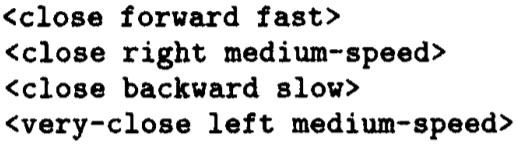
\includegraphics[scale=0.7]{images/musto}
		\caption{The hypothesized qualitative representation with the left most value being the distance, followed by the direction to move in and finally the speed with which to move \cite{musto1999qualitative}.}
		\label{fig:musto}
	\end{figure}
	
	
	\paragraph{Conclusion}Since this \cite{musto1999qualitative}, is another teach-replay approach its major drawback is the over-reliance on the teach phase, furthermore being a teach replay approach that utilizes sonar distances, angles and dead reckoning to obtain trajectories, the system cannot deal with dynamic objects such as humans that may be encountered during autonomous replay as these objects did not exist during the teach phase and hence no information about them exists in the systems knowledge of the environment. The authors also fail to provide concrete information regarding how the control decisions are made instead choosing to only mention that this is done based on the differences in the represented trajectories. One clear merit of this implementation was the hypothesis of how qualitative distance and direction calculi can be combined to achieve navigation in robots, but this is also its drawback as this was only hypothesized and not tested or implemented on the mobile platform. Again the authors assume better efficiency in terms of power consumption and computational requirements due to the usage of qualitative representations yet they fail to provide any conclusive evidence as validation.

	\paragraph{}The approach presented in \cite{sgouros2002qualitative} makes use of a unique qualitative map based representation, which is inherently based on distance relations. The authors propose the `Qmap' framework which accepts as an input a line segment representing the desired path. This line segment is then quantized into rectangular cells that form a part of the grid. Since the robot is equipped with a sensor array of 8 sonars each placed at 45 degrees (in a manner similar to the layout of the cardinal directions) and orientation sensors the data received from each of these sensors is stored in a qualitative manner within the cells of the grid. Sensors that are in close proximity of obstacle are marked as active and their respective relations are indicated using either of the three distance primitives [I(increasing), D(decreasing), S(stable)], this is the qualitative data that is stored in each cell during the off-line planning phase. During the run-time the implementation takes as input the generated `Qmap' and the starting and ending positions. Additionally, data stored in each cell is compared with the real-time data and the control decisions are made based on the differences between the two. In cases where the difference between the reference data (simulated during the planning stage ) and the real-time data is large such that can be caused by the presence of moving obstacles the preference in the control algorithm is given to the real time data such that it ensures that the robot stops moving completely until further intervention by a human controller.
	\begin{figure}[h]
		\centering
		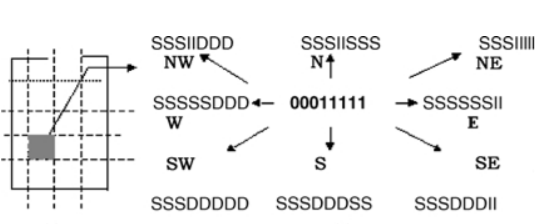
\includegraphics[scale=0.7]{images/Qmap}
		\caption{figure showing the `Qmap' for a given line segment, the 0's and 1's indicate the inactive and active sensors while `S', `I', `D' indicate the distance relations of each sensor w.r.t the obstacle(grey cell) \cite{sgouros2002qualitative}.}
		\label{fig:qmap}
	\end{figure}
	
	\paragraph{Conclusion}The authors mention that the implementation \cite{sgouros2002qualitative}, deals with obstacles by marking those respective cells as blocked, but do not indicate how or when (planning or run-time) this information is provided to the map also the stopping of the robot when dealing with moving objects is an obvious drawback when considering real world applications. The authors mention that a successful navigation was achieved in 60 percent of the cases out of a possible 15 experimental runs, with the causes of failure being the large size of the robot which in turn caused collisions when turning, the accumulation of errors in the orientation data due to inaccurate orientation sensors and errors in localizing the robot position on the `Qmap' due to increasing uncertainty, especially when moving in large open spaces. Yet again the authors mention the efficiency based benefits of the qualitative approach but do not provide tangible proof for it and although this is a promising qualitative representation in relation to a global map of the environment it still does not use any of the traditionally accepted qualitative calculi.
%	\begin{figure}
%		\centering
%		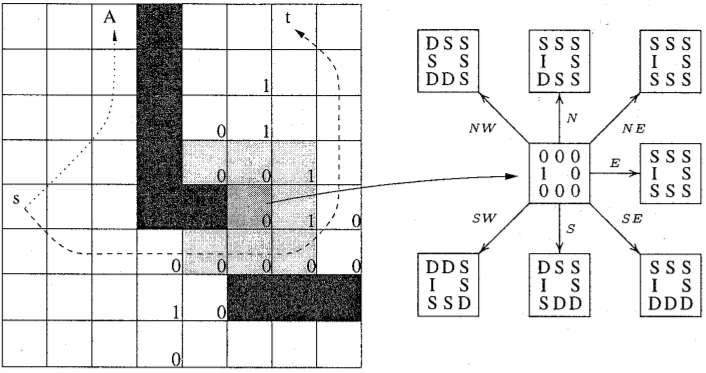
\includegraphics[scale = 0.5]{images/qmap2}
%		\caption{a more descriptive version of the qmap.\cite{vlassis1996global}.}
%		\label{fig:qmap2}
%	\end{figure}
	
%	\item \cite{vlassis1996global}, from this paper we know that the qmap is basically an occupany grid that indicates the free and non-free cells which further include some additional information.
	 \paragraph{}This implementation \cite{shah2011robust}, also provides reasonable cause to prove the utility of qualitative representations in global planners. It uses as an input a hand-drawn map containing the desired path to be followed and a set of landmarks that can be used as a reference. This qualitative map does not have to be accurate but should be able to represent the approximate positions of the landmarks in the physical space. The planning module used in this approach utilizes this approximate way-point positions and the corresponding landmark positions to plan a valid path that can be further fed to a path following module which in-turn executes it on a low level. The path planning is modeled as a quadratic optimization problem, wherein each way-point is influenced by its surrounding landmarks, such that the closest landmark has a higher bearing on the placement of the way-point rather than a landmark that is farther away. The uncertainty in the position of the landmark is also taken into account when placing a way-point in the final trajectory that is to be executed. Furthermore when planning the final path the relative qualitative relations between the robot and the landmarks are maintained which makes it easier to localize the robot based on the available landmarks and in-turn reduce the uncertainty in the positions of the landmarks themselves. Additionally the EKF-SLAM algorithm is used to make the localization and way-point planning more robust.

	\begin{figure}[h!]%
		\centering
		\subfloat[Landmarks (shown as red triangles) represented with linear springs to the proposed waypoint location (shown as a star). For each landmark, the spring constant  is calculated as a function of the distance between waypoint and landmark, and the uncertainty in the estimated location of the landmark (represented by red ellipses) \cite{shah2013qualitative}.]{{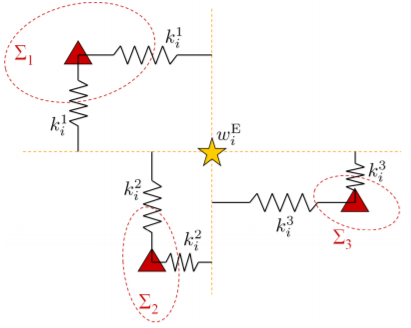
\includegraphics[width=6cm]{images/mappy} }}%
		\qquad
		\subfloat[The sketched map (blue, on left) includes six landmarks and a trajectory that slaloms between pairs of landmarks. In the true environment (red, on right), the robot must slalom more aggressively to pass between
		the landmark pairs \cite{shah2011robust}.]{{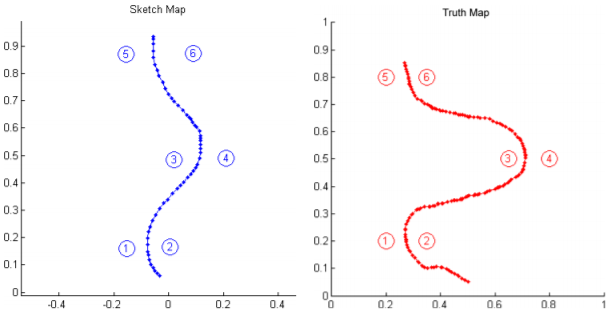
\includegraphics[width=6cm]{images/mappy2} }}%
		\label{fig:hand drawn map}%
	\end{figure}
	\paragraph{Conclusion} This implementation \cite{shah2011robust}, represents a more reliable approach to the utilization of qualitative representations in a global planning based approach. The preservations of qualitative relations between the way-points and the landmarks combined with a SLAM implementation provide a robust platform on which the robot can securely navigate a given environment. In its current state this approach lacks the knowledge of obstacle avoidance for both stationary and mobile objects, also the authors do not elaborate on how the robot knows which observed landmark is to be associated with which reference position in the given map, although during implementation on a robot this problem was solved using a overhead camera this does not suggest a feasible real-time implementation. Furthermore the authors suggest the advantage in efficiency that qualitative approaches have over quantitative approaches but do little to prove this as the truth.
	
%	\item \cite{dondrup2015computational}, This approach utilizes the QTC to analyze human robot spatial interactions and is an extension of the research presented in \cite{hanheide2012analysis}. The study introduces a new variant of the calculi called the $QTC_{BC}$, which is basically a combination of the $QTC_B$ and the $QTC_C$ calculi merged together such that the representation can switch between the two based on a distance threshold. The distance threshold is defined to make a distinction between qualitative social spaces of a human subject such as personal space and close space 
	 \paragraph{}This implementation \cite{bellotto2012robot}, features the use of the qualitative trajectory calculus to create abstractions of human movements and then use these abstractions to reason and execute the corresponding motions of the robot. $QTC_B$ is the selected calculi for creating these abstractions, since it takes into account the relative motion between two mobile objects. The abstractions have been described in detail in the previous section of `Qualitative trajectory calculus'. Using these previously described abstractions the relative motion between the robot's and the human trajectory is encoded as a qualitative representation. A graph structure is used to build a situation graph tree where each node represents a particular scenario or agent's states and the edges indicate the transition to the next possible states. A depth first approach is used to traverse the whole tree and a fuzzy-logic based interpreter(F-Limette) is used to  interpret the states and convert them to a low-level motion command. For the sake of simplicity the authors have only implemented this approach in a restricted limited manner, wherein the robot either follows the human or stops following it based on the described qualitative scenarios.
	\begin{figure}[h]
		\centering
		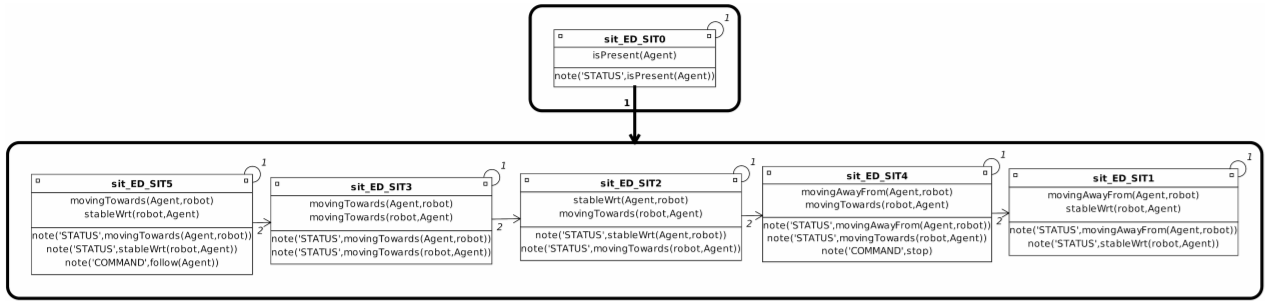
\includegraphics[scale = 0.6]{images/graph}
		\caption{Situation Graph Tree of the human motion behaviour and relative robot actions \cite{bellotto2012robot}.\textcolor{blue}{explain the state and transitions}}
		\label{fig:graph}
	\end{figure}
	
	\paragraph{Conclusion} The above mentioned approach \cite{bellotto2012robot}, was successfully implemented on the robot platform using laser range finders to track human feet, and create suitable abstractions. Yet it presents only a limited view on the applicability of qualitative representations for robot navigation, furthermore when using such graph structures the space and time complexity increases exponentially with increase in the number of scenarios. Thus contradicting the base assumption that using qualitative representations allow improvement to the computational efficiency for a given task. The authors do suggest the improvement of the current approach by replacing the $QTC_B$ representation with a $QTC_C$ representation that allows a finer control paradigm since it includes directional information(left-right) to be represented in addition to the nature of the existing motion(moving away-towards). Although this implementation shows the utilization of the QTC calculi, it cannot be considered a robust implementation due to the lack of extensive testing and the limited experimentation that was carried out for this purpose.
	
	 \paragraph{}This approach \cite{dondrup2016qualitative}, makes use of the qualitative trajectory calculus to depict relative motion between a human and a robot, in a restricted environment which in this case is a corridor. The use of qualitative representations to achieve robot trajectories that are perceived as safe and intuitive by humans is the main aim of this project and to that effect the `pass-by'(human and robot cross each other in opposite directions) scenarios are evaluated. The authors use `velocity costmaps based on the qualitative descriptions to limit the sample space of the dynamic window approach local planner to generate trajectories' \cite{dondrup2016qualitative}, that are safe for the robot and human as well as intuitive for the human. The authors combine the $QTC_B$ and $QTC_C$ calculus into a single calculus called the $QTC_{BC}$ which allows the representation to switch between the $QTC_B$ and $QTC_C$ depending upon a distance threshold. This distance threshold is defined such that when the robot is in close proximity to the human agent the representation switches to $QTC_C$ as this provides a more informed representation of the relative trajectories at farther distances since it is sufficient to know whether the two objects are approaching each other or not, the $QTC_B$ representation is used. 
	\begin{figure}[h]
		\centering
		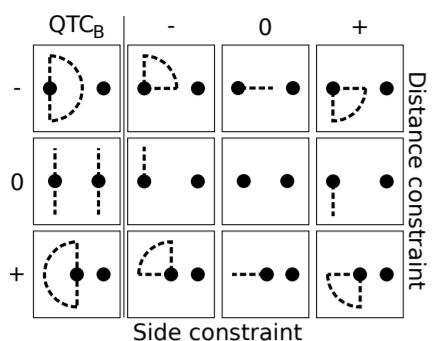
\includegraphics[scale = 0.7]{images/qtcbc}
		\caption{The velocity costmap prototypes. The area enclosed by the partial circle represents the low cost area, everything outside is assigned the highest cost value. The black dot on the right represents a human that can have any possible QTC state (except for $QTC_B$) \cite{dondrup2016qualitative}.}
		\label{fig:qtcbc}
	\end{figure}
	
	
	\paragraph{Conclusion}The approach \cite{dondrup2016qualitative}, was tested by both simulation and application on a robot and the qualitative representation velocity costmaps far outperformed (in terms of minimum number of collisions) the costmaps that utilized Cartesian coordinates as well as a naive dynamic window approach. This approach provides a concrete argument to the utility of qualitative representations in robot navigation as well as human robot interaction, yet it does not clarify the claim stating that the use of qualitative representations is more efficient when compared to a quantitative representation. Also, its evaluation on a single test scenario makes it likely that this approach is highly tuned to achieve greater success on the described task with no indication of its performance on a more generalized task such as navigation through a corridor with or without multiple obstacles.


\section{Limitations of previous work}
\paragraph{} The previous section brings to light a variety of implementations that utilize qualitative spatial representations in varying capacity to abstract spatial entities and relate them in a semantically cohesive manner. The concern that's highlighted immediately is that many of these approaches do not utilize the traditionally accepted qualitative calculi(based on a set of relations, which have been abstracted from underlying mathematical theories and offer a reliable method to describe spatial configurations \cite{lucke2011streets}.) and hence often end up with provisional implementations that have been developed with reliance on a set of highly specific parameters, which if varied will most likely cause the developed algorithm to fail the given task. Thus showing that there is a lack of a generalized approach to the application of qualitative spatial representations in the domain of mobile robot navigation.

\paragraph{} Furthermore all the approaches state the efficiency gain especially in terms of computation and power consumption as the motivation behind using qualitative spatial representations over quantitative ones, but none of them provide tangible proofs to establish the truth of this statement. There exists a lack of effort on this front as there are no comparative studies nor any empirical evidence to support this seemingly obvious claim. 

\paragraph{} Thus for the purpose of this project we will aim to address the above mentioned limitations, in the proposed approach.
